% !TeX spellcheck = en_GB
Heterogeneous computer systems, such as traditional CPU-GPU based systems, 
% keep it simple and remove:
% require different programming models for
% different execution unit types, and they often 
often expose disjoint memory spaces to the programmer,
such as main memory and device memory, with the need
to explicitly transfer data between these.
% \TODO{I was confused with the next 3 sentecnes , please check this version}
The different memories usually 
require different memory access operations and
different pointer types. % on CPU and accelerator side.
% Done, removed the rest as it might confuse:   even in programming
% environments where a single-source program
% involves both CPU and accelerator code.
Also, encoding memory transfers as message passing communications
leads to low-level code that is more error-prone. 
% While the former problem is often solved by 
% compiler support (as in OpenACC, OpenMP4.5 and
% domain-specific languages)
% or other high-level programming
% abstractions (e.g.\ skeleton programming as in 
% SkePU or SkelCL), e.g. 
A commonly used software technique to abstract away the
distributed memory, the explicit message passing,
and the asymmetric memory access mechanisms
consists in providing the programmer with an 
object-based shared memory emulation. For CPU-GPU systems,
this can be done in the form of special data-containers,
which are generic, STL-like data abstractions such as 
\verb+vector<...>+ that 
% \TODO{I am a bit confused with the ``wrap aggregate''} 
% is multi-element better?
wrap multi-element data structures such as arrays. These 
data-container objects
 internally perform transparent, coherent
software caching
of (subsets of) accessed elements in the different memories 
so they can be reused (as long as not invalidated) 
in order to
avoid unnecessary data transfers. Such data-containers 
(sometimes also referred to as ''smart'' containers as they can
transparently perform data transfer and memory allocation optimizations
\cite{Dastgeer-IJPP15}) 
are provided in a number of programming frameworks 
for heterogeneous systems, such as
StarPU \cite{StarPU} and SkePU~\cite{Enmyren10,Dastgeer-IJPP15}. StarPU is a 
C-based library that provides API functions to
define multi-variant tasks for dynamic scheduling
where the data containers are used for modeling 
the operand data-flow
among the dynamically scheduled tasks. 
SkePU defines device-independent 
multi-backend skeletons like map, reduce,
scan, stencil etc.\ where operands are
passed to skeleton calls within data containers.

VectorPU \cite{VectorPU-2017} is a recent C++-only
open-source
programming framework for CPU-GPU heterogeneous systems. 
VectorPU relies on the specification of 
\textit{components}, which are functions that contain kernels for execution
on either CPU or GPU. Programming in VectorPU is thus not restricted 
to using predefined skeletons like SkePU, 
but leads to more high-level and more concise code than StarPU. 
Like StarPU, VectorPU requires the programmer
to annotate each operand of a component
%\TODO{passed to components? (I find the ``operand'' a bit abrupt here)} 
with the access mode (read, write, or both) including the 
accessing unit (CPU, GPU), and uses smart data containers for automatic transparent
software caching based on this access mode information.

The implementation of VectorPU makes excessive use of static metaprogramming; this provides a light-weight realization of the access mode annotations and of the software caching, 
which only require a standard C++ compiler. Emulating these 
light-weight
component and access mode constructs without additional language
and compiler support (in contrast to, e.g., OpenACC or OpenMP), 
leads however to some compromises concerning the possibility to perform static analysis.
In particular, VectorPU has no explicit type system for the
access modes, as these are not known to the C++ compiler.

In this paper, we  formalize access modes
and data transfers in CPU-GPU heterogeneous systems and prove 
the correctness of the software
cache coherence mechanism used in VectorPU.
The contributions of this paper are:

\begin{itemize}
\item A simple effect system modeling the semantics of memory
   accesses and communication in a CPU-GPU heterogeneous system,
\item A small calculus expressing different memory
   accesses and their composition across program traces. 
\item The interpretation of VectorPU operations as higher-level statements
    that can be translated into the core calculus,
\item A proof that, if all memory accesses are performed 
    through VectorPU operations, the memory cannot reach an 
    inconsistent state and all memory accesses succeed,
\item The abstraction necessary to take into account arrays, possibly overlapping, in the formalism.
\end{itemize}

This article is an extended version of \cite{HKL-4PAD2018}, with two main additions. First the relationship between the formal results and the VectorPU implementation is  detailed, illustrating the impact of the proven results on the behaviour of the library. Second, the theoretical framework is extended to take into account the fact that manipulated arrays may overlap and that the consistency mechanism must take this information into account to be correct. While overlapping arrays are not yet supported by VectorPU, based on the formal model we develop, we show how a simple extension of the library could provide support for overlapping arrays.

This paper is organized as follows:
Section~\ref{VectorPU} reviews VectorPU as far as required for  this paper, for further information we refer to \cite{VectorPU-2017}.
Section~\ref{sec:Formal} provides our formalization of VectorPU programs and
their semantics, and proves that the coherence mechanism used in
VectorPU is sound. Section~\ref{sec:RW} discusses related work, and 
Section~\ref{sec:conclusion} concludes.

\begin{figure}
\begin{center}
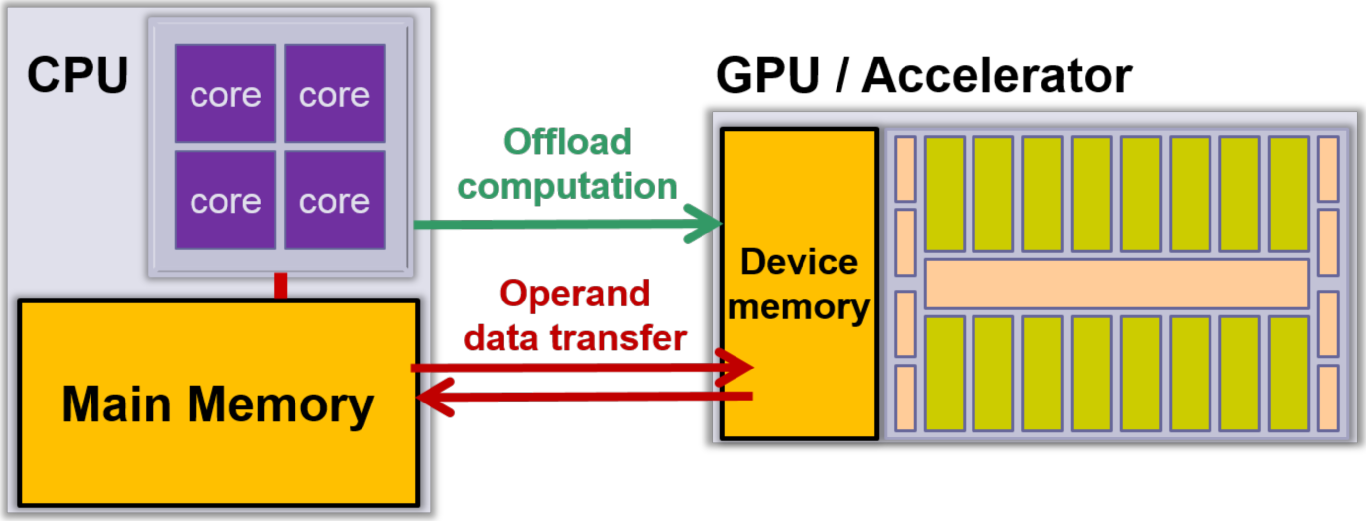
\includegraphics[width=0.64\textwidth]{img/CPU-GPU.png}
\caption{\label{fig:CPU-GPU}A GPU-based system with distributed address space}
\end{center}
\end{figure}

\section{VectorPU}\label{VectorPU}

In heterogeneous systems with separate address spaces, for example in 
many GPU-based systems, a general-purpose processor
(CPU) with direct access to main memory is connected by some network
(e.g., PCIe bus) to one or several accelerators
(e.g., GPUs) each having its own device memory,
see Figure~\ref{fig:CPU-GPU}. Native programming models
for such systems such as CUDA typically expose the distributed address spaces to the programmer, who has to write explicit 
code for data transfers and device memory management.
Often, programs for such systems  must be organized in multiple source files
as different programming models and different toolchains
are to be used for different types of execution unit.
This enforces a low-level programming style. 
Accordingly, a number of single-source 
programming approaches have been proposed that abstract away the distribution 
by providing a virtual shared address space. Examples include directive-based
language extensions such as OpenACC and OpenMP4.5, and C++-only approaches 
such as the library-based skeleton programming framework SkePU \cite{Dastgeer-IJPP15}
and the recent macro-based framework \textit{VectorPU}.

\textit{VectorPU} \cite{VectorPU-2017} is an open-source\footnote{http://www.ida.liu.se/labs/pelab/vectorpu, https://github.com/lilu09/vectorpu} lightweight C++-only 
high-level programming layer
for writing single-source heterogeneous programs for Nvidia CUDA GPU-based systems.
Aggregate operand data structures 
passed into or out of  function calls are
to be wrapped by special data containers known to VectorPU.
VectorPU currently provides one generic data container,
called \verb+vector<...>+,
with multiple variants that 
eliminate the overhead of managing heterogeneity and distribution when not required (e.g., when no GPU is available). 
\verb+vector<...>+ inherits functionality from STL \verb.vector. 
and from Nvidia Thrust \verb.vector., and
wraps a C++ array allocated in main memory. 
VectorPU automatically creates on demand
copies of to-be accessed elements in device memory and keeps all copies coherent using
a simple coherence protocol, data transfers are only performed when needed. 

VectorPU programs are organized as a set of C++ functions, some of which
might internally use device-specific programming CUDA constructs\footnote{%
VectorPU allows to directly annotate a CUDA kernel function, in addition to annotating its C++ wrapper function.} while others
are expected to execute on the host, using one or possibly multiple cores.
VectorPU \emph{components} are functions that are supposed to contain (CPU or device)
kernel functionality and for which  operands are passed as VectorPU data container objects. 
Components and the types of execution units that
access their operands are declared 
by annotating the operands of the function, either at a call of the function
or for the formal parameters in the function's declaration, 
with VectorPU \emph{access mode specifiers}. For example, in contrast,  SkePU \cite{Enmyren10}  overloads element
access and iterator operations so that monitored 
accesses are also possible on demand in non-componentized (i.e., 
ordinary C++) CPU code.
VectorPU only relies on access mode annotations 
to perform lazy data transfer,
not knowing when data is going to be accessed inside a component.
% however, SkePU knows by overloading element accesses.
% By overloading element
% access and iterator operations, 

Table~\ref{tab:modes} summarizes the access mode annotations
currently defined for VectorPU. The access mode specifiers,
such as \texttt{R} (read on CPU), \texttt{W} (write on CPU), \texttt{RW} 
(update, i.e., both read and write, on CPU), \texttt{GR} (read on GPU) and so forth,
are available both as annotations of function signatures and
as C++ preprocessor macros that expand at compilation into (possibly, device-specific) C++ pointer
expressions and side effects that allow to generate device specific access code
and use device-specific pointer types for the chosen execution unit. 
For instance, \texttt{GW(x)} expands to a GPU pointer to
the GPU device copy of \texttt{x},
which might be dereferenced for GPU writing accesses to \texttt{x},
such as the GPU code: \verb:*( GW(x) + 2 ) = 3.14:.
\texttt{GWI(x)} evaluates to a Thrust-compatible iterator onto the 
GPU device copy of \texttt{x}, and \texttt{WEI(x)} to an iterator-end reference
to the last element of \texttt{x} on CPU side. The current VectorPU prototype implementation does not
(yet) check access-mode annotations in signatures of externally defined functions.
%
It is also possible to specify partial access of a \verb:vector:
% that expand into pointers to the first and last element
% of an interval of elements to be accessed, 
instead of the
entire \verb.vector. data structure. The current
VectorPU implementation does not (yet) support coherence for 
\emph{overlapping}
intervals of elements resulting from multiple (partial) accesses
some of which (may) access the same element.
A solution for this problem has been described for SkePU
smart containers by Dastgeer~\cite{Dastgeer-IJPP15}. Section~\ref{sec:overlap-array} details a solution for handling overlapping arrays in VectorPU.
%


\begin{table}
\caption{\label{tab:modes}VectorPU access mode annotations for a parameter  \cite{VectorPU-2017}}

\begin{center}
\begin{tabular}{|lll|}
\hline
Access Mode & On Host & On Device \\
\hline
Read pointer & \texttt{R} & \texttt{GR} \\
Write pointer & \texttt{W} & \texttt{GW} \\
Read and Write pointer & \texttt{RW} & \texttt{GRW} \\
Read Iterator & \texttt{RI} & \texttt{GRI} \\
Read End Iterator & \texttt{REI} & \texttt{GREI}\\
Write Iterator & \texttt{WI} & \texttt{GWI}\\
Write End Iterator & \texttt{WEI} & \texttt{GWEI}\\
Read and Write Iterator & \texttt{RWI} & \texttt{GRWI}\\
Read and Write End Iterator & \texttt{RWEI} & \texttt{GRWEI}\\
Not Applicable & \texttt{NA} & \texttt{NA} \\
\hline
\end{tabular}
\vspace{-3ex}
\end{center}
\end{table}


The following example (adapted from \cite{VectorPU-2017}) 
of a CUDA kernel wrapped in an 
 annotated function \verb.bar. shows the use of 
VectorPU access mode annotations at function declaration:

{\footnotesize \begin{verbatim}
// Example (annotations at function declaration): 
__global__
void bar ( const float *x [[GR]], float *y [[GW]],
                 float *z [[GRW]], int size )
{ ... CUDA kernel code ... }
\end{verbatim}}

Here, the operand array pointed to by \verb.x. may be read (only) by the GPU within \verb.bar.,
operand array \verb.y. must be written (only) by the GPU, and 
operand array \verb.z. may be read and/or written by the GPU.
When calling \verb.bar., the
first three operands are  passed as VectorPU \verb.vector. 
container objects.
The \verb.size. formal parameter is a scalar (not a data container), so it
will be available on GPU on a copy-in basis but no coherence will
be provided for it by VectorPU.

It is also possible to put the annotations into a call, and hence characterize a function as a VectorPU component:


{\footnotesize \begin{verbatim}
// declare a CPU function:
void foo ( const float *x, float *y, float *z, int size );

// declare three vectors:
vectorpu::vector<float> vx(100), vy(100), vz(100);

// call to VectorPU annotated function foo:
foo ( R( vx ), W( vy ), RW( vz ), size ) ;
\end{verbatim}}

Here, the access mode specifiers and the resulting coherence policy
 only apply to that particular invocation of \verb-foo-, while other
invocations of \verb-foo- might use different access mode specifiers.

The following example shows how to use iterators:

{\footnotesize \begin{verbatim}
vectorpu::vector<My_Type> vx(N);
std::generate( WI(vx), WEI(vx), RandomNumber );
thrust::sort( GRWI(vx), GRWEI(vx));
std::copy( RI(vx), REI(vx), ostream_iterator<My_Type>(cout, ""));
\end{verbatim}}

\noindent 
where \verb.std::generate. is a CPU function filling a section between
two addresses with values (here, random numbers),
and \verb.thrust::sort. denotes the GPU sorting functionality
provided by the Nvidia Thrust library. 

% CK 190926: moved to new subsection 2.1 on pvectors
% % New 180916 CK:
% Using iterators, it is possible to define, in VectorPU, references to
% contiguous subranges of a vector,
% called \textit{partial vectors} (\texttt{pvector}s), 
% which can be passed as \texttt{vector}-compatible
% operands to a function instead of an entire \texttt{vector}.
% In this way, it is possible to pass several (disjoint or even
% overlapping) \texttt{pvector} objects as seemingly different \texttt{vector}
% arguments that however are just windows onto
% a common \texttt{vector} container variable. 




% CK new 190127 text from LL:

\subsection{Partial Vectors}
%{{{
\label{sec:Partial Vectors}

% first paragraph replaced by old pvector description below:
%To cope with functions that operate on only a regular part of a normal VectorPU vector
%efficiently, VectorPU provides a specialized kind vector called partial vector,
%that can represent a partial range of a normal vector.

% New 180916 CK:
Using iterators, it is possible in VectorPU to define references to
contiguous subranges of a vector,
called \textit{partial vectors} (\texttt{pvector}s), 
which can be passed as \texttt{vector}-compatible
operands to a function instead of an entire \texttt{vector}.
In this way, it is possible to pass several (disjoint or even
overlapping) \texttt{pvector} objects as seemingly different \texttt{vector}
arguments that however are just windows onto
a common \texttt{vector} container variable. 
In contrast to \texttt{vector}s without \texttt{pvector}s, where coherence is 
managed automatically by VectorPU, the coherence 
management in the presence of \texttt{pvector}s 
is exposed to the programmer.

A partial vector can be initialized by two iterators to a normal VectorPU \texttt{vector} (we call it \emph{mother vector}).
% representing the convex closure of the index ranges of
% all contained partial vectors. 
No new memory is allocated for this partial vector, 
only the two iterators are stored, 
and the coherence state for its range in the mother vector.
% for the range of data this partial vector contains.
When a partial vector is declared, it automatically
inherits the coherence state information
from its mother vector. 
% already said above:
% Afterwards, VectorPU algorithms can operate on the initialized partial vector
% in the same way as for other VectorPU vectors.

\begin{figure}
\noindent 
\begin{minipage}{\linewidth}
\begin{footnotesize}% changed from small to have same font size as in other code snippets
\begin{verbatim}
struct my_set {
   template <class T>
   __host__ __device__
      void operator() (T &x) { x+=101; } 
};
vectorpu::vector<int> vx(10);  // the mother vector
vectorpu::pvector<int> vy(x, vx.begin(), vx.begin()+2);
vectorpu::for_each<int>( GWI(vy), GWEI(vy), my_set() );
vectorpu::for_each<int>( GWI(vy), GWEI(vy), my_set() );
SR( vy );  // explicit coherence management
vectorpu::for_each<int>( RI(vx), REI(vx), [](auto x) {cout<<x<<" ";} );  
\end{verbatim}
\end{footnotesize}
\end{minipage}
\caption{\label{fig:pvector}Example of using a partial vector (\texttt{pvector}) and the \texttt{SR} macro for explicit coherence management. (Note: \texttt{pvector} is a short form and actually called \texttt{parco\_vector} in the VectorPU API.)}
\end{figure}

% One important point to make this mechanism work is for the case 
The aliasing introduced by \texttt{pvectors} can lead to coherence problems. One such scenario could be that the
programmer intends to operate on the previous \texttt{vector} again after
some part of it was updated via a \texttt{pvector}, 
hence the whole \texttt{vector} would be in an inconsistent state.
In such cases, VectorPU expects the programmer to use a macro \texttt{S$X$} (\texttt{S}ynchronize for access mode $X$,
such as \verb.SR. for synchronized read)
just before the programmer operates on the whole vector again.
It may be inefficient for a \texttt{pvector} to perform the \texttt{S$X$} synchronization
automatically, because multiple operations can be performed on the same \texttt{pvector} 
before accessing the whole \texttt{vector} again, 
and because the \texttt{pvector}
has no knowledge about when the operations on itself will be finished, hence
keeping them coherent each time is not necessary and thus a waste of performance.

% Listing~\ref{lst:parco_vector} 
Figure~\ref{fig:pvector}
shows an example of using a \texttt{pvector} and the 
\texttt{S$X$} macro.
It initializes a mother vector \texttt{vx}
and a \texttt{pvector} \texttt{vy} on it.
The following two lines change part of \texttt{vy}'s value multiple times. % by operating on the \texttt{pvector}
%using the functor in Listing~\ref{lst:skeleton_programming}.
The \texttt{SR} macro explicitly restores coherence for
\texttt{vy} before the following read access, 
resulting in a write-back of \texttt{vy} elements in GPU device memory
to their locations in \texttt{vx},
% only once for the multiple changes partially, 
thus also \texttt{vx} as a whole becomes coherent again
and line 6 is safe to operate on the whole \texttt{vx}.

% CK: I do not understand this, dropped for now.
% For applications in which the workload changes dynamically from one iteration to another,
% e.g.\ a parallel reduction on GPU where the workload 
% shrinks by half at each iteration,
% it is possible to initialize \texttt{pvector}s dynamically.
% Hence, when switching to a CPU implementation 
% as the workload is small enough,
% the partial data get coherence-managed automatically
% by VectorPU.
%}}}



\begin{figure}[tb]
\begin{minipage}{.48\textwidth}
\begin{small}
\begin{verbatim}
void coherent_on_cpu_r(){
  	 if( !cpu_coherent_unit ){
       download();
       cpu_coherent_unit=true;
  	 }
}
void coherent_on_cpu_w(){
  	 cpu_coherent_unit=true;
  	 gpu_coherent_unit=false;
}
void coherent_on_cpu_rw(){
  	 if( !cpu_coherent_unit ){
       download();
       cpu_coherent_unit=true;
  	 }
  	 gpu_coherent_unit=false;
}
\end{verbatim}
\end{small}
\end{minipage}\qquad~
\begin{minipage}{.48\textwidth}
\begin{small}
\begin{verbatim}
void coherent_on_gpu_r(){
  	 if( !gpu_coherent_unit ){
       upload();
       gpu_coherent_unit=true;
	 }
}
void coherent_on_gpu_w(){
  	 gpu_coherent_unit=true;
  	 cpu_coherent_unit=false;
}
void coherent_on_gpu_rw(){
  	 if( !gpu_coherent_unit ){
       upload();
       gpu_coherent_unit=true;
  	 }
  	 cpu_coherent_unit=false;
}
\end{verbatim}
\end{small}
\end{minipage}
\caption{\label{fig:vectorpucoherence}Coherence control code,
    here for simple vectors,
    in \texttt{vectorpu.h}. Functions \texttt{download} and
    \texttt{upload} are implemented using CUDA
    \texttt{thrust::copy}. Validity of copies on CPU and GPU
     is indicated
     by the flags \texttt{cpu\_coherent\_unit} and
     \texttt{gpu\_coherent\_unit} respectively; both are
     initialized to \texttt{true}
     in code allocating new vectors (not shown).}
     % 
     % for the records:
     %
     % template <class T, class Index_Type=std::size_t>
     % struct min_vector : public std::vector<T>, public thrust::device_vector<T> {
     % explicit min_vector(Index_Type _array_size):
     %  	 std::vector<T>::vector(_array_size),
     %  	 thrust::device_vector<T>::device_vector(_array_size),
	 % cpu_coherent_unit(true),
	 % gpu_coherent_unit(true),
     %  	 array_size(_array_size),
     % start_pos(0) {}
\end{figure}




%\vspace{1.4mm}
%\noindent
%\textit{Implementation notes }
\subsection{Implementation Notes}

\paragraph{Coherence protocol}
%
In the source code of VectorPU, the code
relevant for our work is the part of \verb+vectorpu.h+%
\footnote{The VectorPU source code can be found at
\texttt{https://github.com/lilu09/vectorpu}.} 
that handles coherence. Its implementation for the various
variants of \texttt{vector} 
(see the code excerpt in Fig.~\ref{fig:vectorpucoherence} for
simple \texttt{vector}s) follows a
simple valid-invalid protocol.
%(single-reader single-writer sharing).

% CK new 190127 - text snippet from LL:
\paragraph{Expansion of macro annotations to device-specific pointers}

For function parameters, the macro annotations expand into appropriate C code to fit their function call context.
For illustration, we show the simplified code after a function parameter's expansion ($\longrightarrow$) for four typical annotations,
where \texttt{vx} refers to a VectorPU \texttt{vector} instance:

\begin{small}
\begin{itemize}
 \item \texttt{R(vx)} $\longrightarrow$ 
 \begin{minipage}[t]{0.8\textwidth}
  \texttt{set\_coherence\_state();}\\
  \texttt{return this->std::vector<T>::data();}\\
  \texttt{//casted as const in return value}
 \end{minipage}
 \item \texttt{W(vx)} $\longrightarrow$ 
 \begin{minipage}[t]{0.8\textwidth} \texttt{set\_coherence\_state();}\\
 \texttt{return this->std::vector<T>::data();}
 \end{minipage}
 \item \texttt{GR(vx)} $\longrightarrow$ \begin{minipage}[t]{0.8\textwidth}
 \texttt{set\_coherence\_state();}\\
 \texttt{return thrust::raw\_pointer\_cast(}\\
 \hspace*{1em}\texttt{\& (* thrust::device\_vector<T>::begin() ) );}\\
 \texttt{//casted as const in return value}
 \end{minipage}
 \item \texttt{GW(vx)} $\longrightarrow$ 
\begin{minipage}[t]{0.8\textwidth} \texttt{set\_coherence\_state();\\ return thrust::raw\_pointer\_cast(}\\
\hspace*{1em}\texttt{\& (* thrust::device\_vector<T>::begin() ) );}
\end{minipage}
\end{itemize}
\end{small}

Hence, each annotated parameter is expanded to some code snippet\footnote{One can think of those code snippets as
anonymous functions or lambda functions. 
In the real scenarios these code snippets are encapsulated within a function,
and each macro as shown above expands to a call to its function.}.
In all scenarios the expanded macros first update the coherence state according to the annotation's semantics.
Then, for the CPU cases, a pointer to a \texttt{std::vector} is returned,
and for the GPU cases, a pointer to a Thrust pointer (which is a pointer to GPU memory space) is returned.
For read-only cases, the return value is casted to \texttt{const} to ensure type safety in its function invocation.
For write-only cases, no such \texttt{const} cast happens.

\paragraph{Partial vector implementation and memory management}
% new 180916 CK:
For implementing the \texttt{pvectors} atop \texttt{vector}s, 
VectorPU uses the simplistic approach of allocating memory for
the \emph{entire} \texttt{vector} on the device 
even if the \texttt{pvector}(s) might only
access a minor part of it. This may waste device memory space 
but makes local address calculations easy, and anyway only
the accessed elements (the \texttt{pvector} range) will be transferred.
As we will see later, it also simplifies coherence management
for \emph{overlapping} \texttt{pvector} accesses, which was not 
really foreseen 	in the original VectorPU design.

% CK new 190127 input from LL:
In order to better utilize the device memory,
a future extension of VectorPU could implement 
\emph{lazy allocation}.
In lazy allocation mode, VectorPU maintains for each 
\texttt{vector} another state
flag called \texttt{is\_allocated}
to track whether it is allocated for host/device memory or not.
When a VectorPU \texttt{vector} is declared,
by default, no device memory is really allocated and the \texttt{is\_allocated} flag is set to false.
Only upon its first use in a function call as an
annotated \texttt{vector} argument,
the flag \texttt{is\_allocated} is checked.
If it is false (not allocated), device memory is allocated,
otherwise, the memory is already allocated and no new memory will be allocated.
Afterwards, the function call continues.

%\vspace{1.4mm}
%\noindent
%\textit{Efficiency }
\subsection{Efficiency}

Using only available C++(11) language features, 
VectorPU provides a flexible unified memory
view where all data transfer and device memory management
is abstracted away from the programmer. Nevertheless,
its efficiency is on par with that of handwritten CUDA code
containing explicit data movement and memory management code
\cite{VectorPU-2017}.
In particular, the VectorPU prototype was shown to
achieve 1.4x to 13.29x speedup over good quality
code using Nvidia's \textit{Unified Memory} API
on several machines ranging from laptops to supercomputer nodes,
with Kepler and Maxwell GPUs. For a further discussion of
VectorPU features, such as
specialized versions of \verb-vector-, for descriptions
of how to use VectorPU together with lambda expressions 
e.g.\ to express skeleton computations, and for further
experimental results 
we refer to \cite{VectorPU-2017}.
